% !TeX spellcheck = en_US
\section{Logistics Regression}

Though named as "regression", logistics regression is used for classification problem, just like Linear Discriminant (\secref{sec:linear-classification}).

\hlb{Problem:} In many of binary classification problems (classification problem with 2 classes), it's rather hard (or even impossible) to be certain about the class of the output, and the training data is not linear separable. Instead of a hard threshold, we could have a soft one, represent by the \ac{prob} belonging to either classes.
\begin{figure}[hbt!]
	\centering
	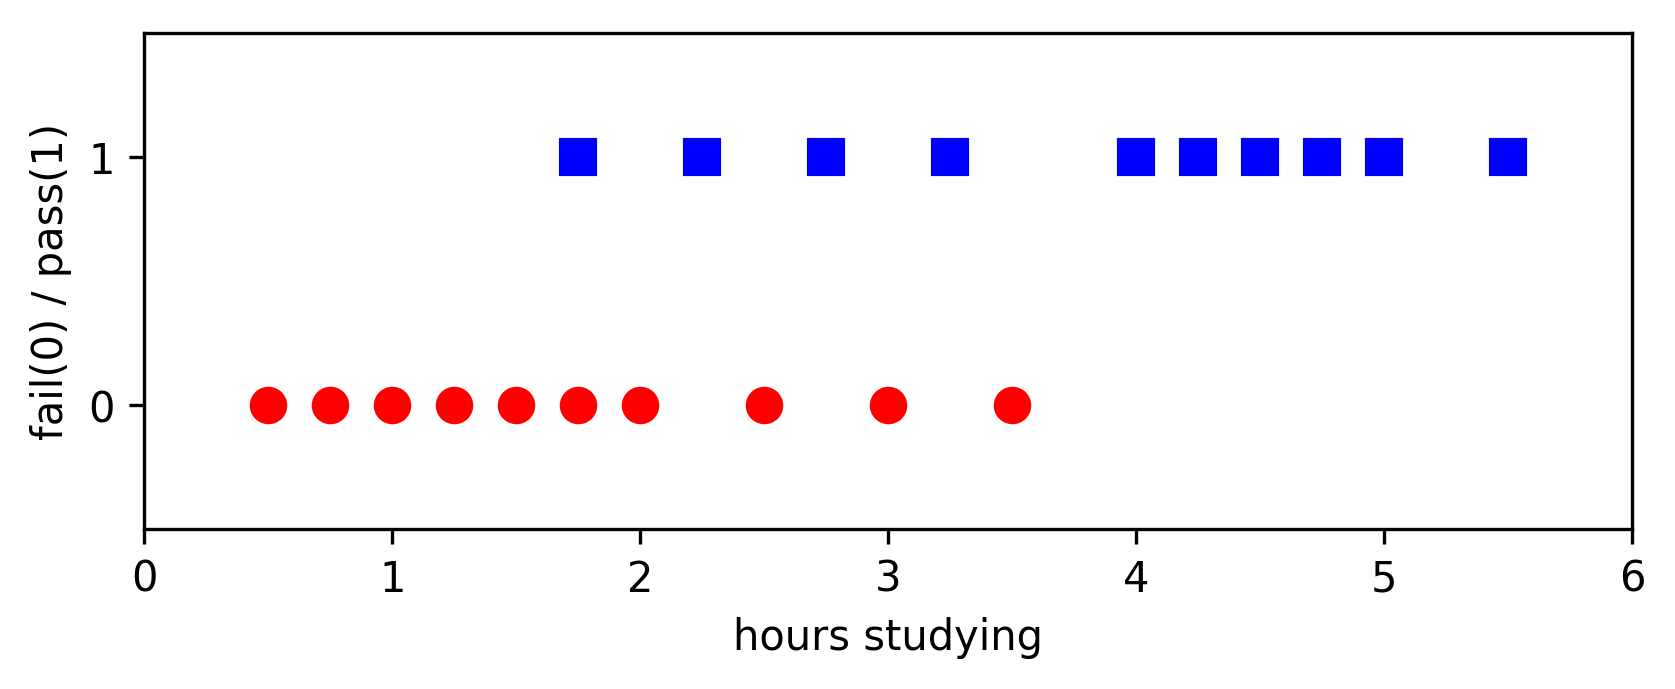
\includegraphics[width=0.79\textwidth]{sigmoid-example.png}
	\caption{Example of exam results based on study hours (\href{https://machinelearningcoban.com/2017/01/27/logisticregression/}{src}). Given the number of hours, instead of predicting whether fail or pass, the model predicts the \ac{prob} that the student will pass, or fail.}
\end{figure}

The sigmoid function gives a nice nonlinear transition for the \ac{prob}. The further the data point is from the threshold, the higher the \ac{prob} it belongs to one class, and small to the others.
\begin{align}
	f(s) 		&= \frac{1}{1 + e^{-s}} \overset{\triangle}{=} \sigma(s) \\
	s 			&= \text{ln} \left( \frac{\sigma}{1-\sigma} \right) \\
	\sigma'(s)	&= \sigma(s) \left( 1- \sigma(s) \right)
	\label{eq:sigmoid}
\end{align}
\begin{figure}[hbt!]
	\centering
	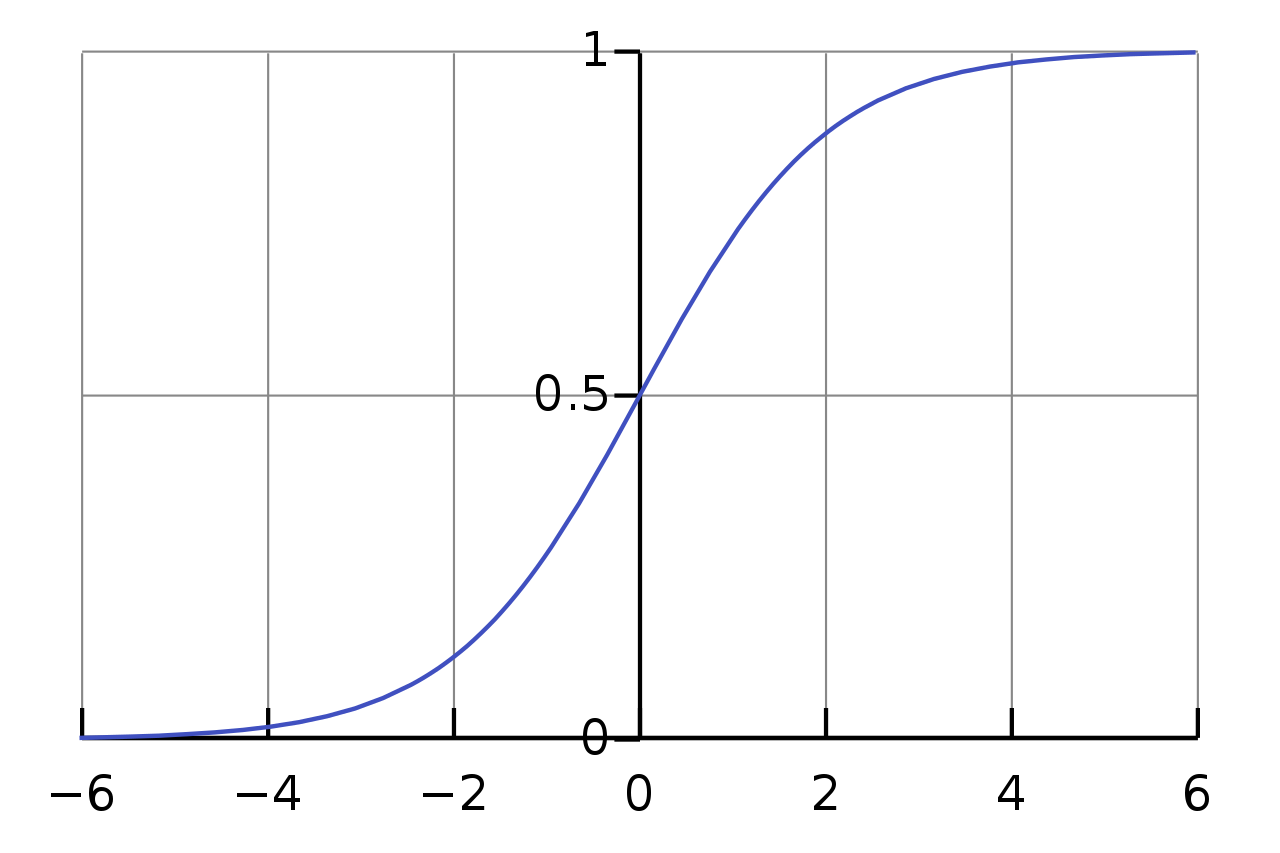
\includegraphics[width=0.5\textwidth]{sigmoid.png}
	\caption{Sigmoid function (\href{https://en.wikipedia.org/wiki/Sigmoid_function}{src}).}
\end{figure}

\hlb{Approach:}
\begin{itemize}
	\item Design of the error function.\\
	Assume that the \ac{prob} of data point $\textbf{x}$ falls into class 1 is $f(\textbf{w}^T\textbf{x})$ and class 0 is $1-f(\textbf{w}^T\textbf{x})$. With $z_i = f(\textbf{w}^T\textbf{x}_i)$:
	\begin{equation}
		\begin{cases}
			P(y_i=1|\textbf{x}_i; \textbf{w}) &= f(\textbf{w}^T\textbf{x}_i) = z_i \\
			P(y_i=0|\textbf{x}_i; \textbf{w}) &= 1 - f(\textbf{w}^T\textbf{x}_i) =1 - z_i
		\end{cases} \Leftrightarrow P(y_i | \textbf{x}_i; \textbf{w}) = z_i^{y_i}(1-z_i)^{1-y_i}
	\end{equation}
	With the aim to find the model \ac{param} that maximizes the data \ac{prob} (\subsecref{subsec:mle}):
	\begin{align*}
		\textbf{w}^* &= \arg \underset{\textbf{w}}{\max}\;P(\textbf{y}|\textbf{X; w}) && \\
		&= - \arg \underset{\textbf{w}}{\min} \log P(\textbf{y}|\textbf{X; w}) && \text{(negative log-likelihood)} \\
		P(\mathbf{y}|\mathbf{X}; \mathbf{w}) &= \prod_{i=1}^N P(y_i| \mathbf{x}_i; \mathbf{w}) = \prod_{i=1}^N z_i^{y_i}(1 - z_i)^{1- y_i} && \text{(independence assumption)} \\
		- \log P(\textbf{y}|\textbf{X; w}) &= - \sum_{i=1}^{N} [ y_i\log z_i + (1-y_1)\log (1-z_i) ] && \text{(the cross entropy error)}
	\end{align*}
	
	\item Optimization with \ac{SGD}:
	\begin{align}
			\textbf{w} &= \textbf{w} - \eta.\frac{\partial J}{\partial x} \tab \text{($\eta$ as the learning rate)}
			\label{eq:log-reg-sgd}\\			
			J(\textbf{w}, \textbf{x}_i, y) &= -\left( y_i\log z_i + (1-y_i)\log(1-z_i) \right), \tab \text{data point $(\textbf{x}_i, y_i)$} \\
			\Rightarrow \; \frac{\partial J}{\partial \textbf{w}} &= - \left( \frac{y_i}{z_i} - \frac{1-y_i}{1-z_i} \right) \frac{\partial z_i}{\partial\textbf{w}} = \frac{z_i - y_i}{z_i(1-z_i)} \frac{\partial z_i}{\partial\textbf{w}} \\
			\frac{\partial z_i}{\partial s} &= z_i(1-z_i) \tab \text{(the beauty of sigmoid function, \eqref{eq:sigmoid})} \\
			\Rightarrow \; \frac{\partial z_i}{\partial\textbf{w}} &= \frac{\partial z_i}{\partial s} \frac{\partial s}{\partial \textbf{w}} = z_i(1-z_i) \frac{\partial(\textbf{w}^T\textbf{x})}{\partial \textbf{w}} = z_i(1-z_i) \textbf{x} \\
			\Rightarrow \; \frac{\partial J}{\partial \textbf{w}} &= (z_i - y_i) \textbf{x}_i\\
			\Rightarrow \; w &= w + \eta (y_i - z_i) \textbf{x}_i \tab \text{(replace into \eqref{eq:log-reg-sgd})}
	\end{align}
\end{itemize}

\note Require less \ac{param}, only $D$ with $D$ as the \ac{no} dimensions, compared to Gaussians with $\displaystyle \left[\frac{M(M+5)}{2}+1\right]$ \ac{param}.

\section{Softmax Regression}

\hlr{Multinomial Logistics Regression, Maximum Entropy Classifier}

\begin{equation}
	a_i = \frac{\text{exp}(z_i)}{\sum_{j=1}^{C}\text{exp}(z_j)}
\end{equation}
so that $\begin{cases}
	a_i > 0 \\
	\sum a_i = 1 \\
	z_m > z_n \iff a_m > a_n \;\;\text{(order)}
\end{cases}$

When $z_i$ is too big
\begin{equation}
	\frac{\text{exp}(z_i)}{\sum_{j=1}^{C}\text{exp}(z_j)} = \frac{\text{exp}(z_i - c)}{\sum_{j=1}^{C}\text{exp}(z_j - c)}
\end{equation}
with $c = \underset{i}{max}\;z_i$

\begin{align}
	&J(w,x,y) = - \sum_{i=1}^{N} \sum_{j=1}^{C} y_{ij}\,\text{log}(a_{ij}) \\
	&J(w,x,y) = - \sum_{n=1}^{N} \sum_{k=0}^{1} \left[ \mathbb{I}(t_n=k)\; \text{ln}\,p(y_n=k | x_n; w) \right] \\
	\Rightarrow &E(w) = - \sum_{n=1}^{N} \sum_{k=1}^{K} \left[ \mathbb{I}(t_n=k)\; \text{ln}\frac{\text{exp}\,(w_k^T x)}{\sum_{j=1}^{K} \text{exp}(w_j^T x)} \right] \\
	&\frac{\partial J_i(w)}{\partial W} = x_i e_i^T = x_i (a_{ij} - y_{ij})^T \\
	&W = W + \eta x_i (y_i - a_i)^T
\end{align}